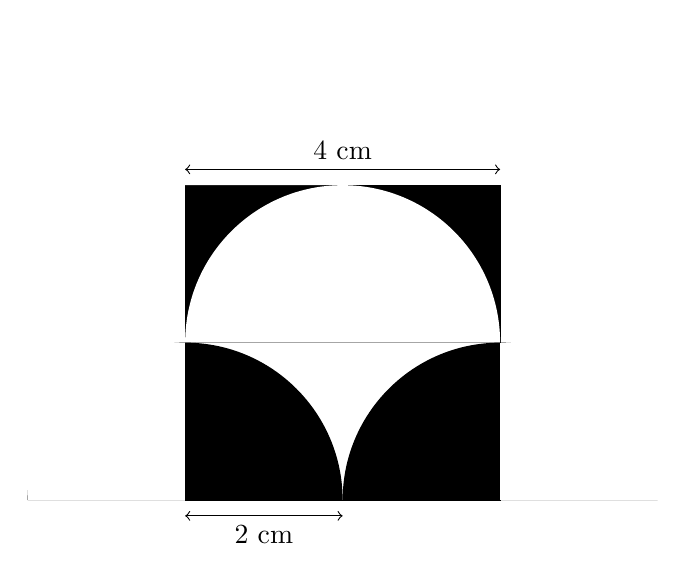
\begin{tikzpicture}
    \draw[fill=white] (0,0) rectangle (4,4);
    \fill[fill=black] (0,2) rectangle (4,4);
    \fill[white] (4,2) arc[start angle=0, end angle=180, radius=2cm] -- cycle;
    \fill[white] (2,4) arc[start angle=0, end angle=180, radius=2cm] -- cycle;
    \fill[black] (2,0) arc[start angle=0, end angle=180, radius=2cm] -- cycle;
    \fill[black] (6,0) arc[start angle=0, end angle=180, radius=2cm] -- cycle;
    \fill[fill=white] (-2,0) rectangle (0,2);
    \fill[fill=white] (4,0) rectangle (6,2);
    \draw[<->] (0,4.2) -- (4,4.2) node[midway, above] {4 cm};
    \draw[<->] (0,-0.2) -- (2,-0.2) node[midway, below] {2 cm};
\end{tikzpicture}

